% !TeX program = pdflatex
% Plantilla breve basada en NTC 1486. Reemplace los datos entre corchetes.
\documentclass[12pt,letterpaper,oneside]{article}

\usepackage[utf8]{inputenc}
\usepackage[T1]{fontenc}
\usepackage[spanish,es-nodecimaldot]{babel}
\usepackage{helvet} % Familia sans serif similar a Arial
\renewcommand{\familydefault}{\sfdefault}
\usepackage[top=3cm,bottom=3cm,left=4cm,right=2cm]{geometry}
\usepackage{setspace}
\onehalfspacing
\usepackage{graphicx}
\usepackage{float}
\usepackage{caption}
\usepackage{enumitem}
\usepackage{hyperref}
\usepackage{fancyhdr}
\usepackage{titlesec}

\graphicspath{{reports/figures/}}
\setlength{\parindent}{0pt}
\setlength{\parskip}{6pt}
\setlist{nosep,leftmargin=*}
\captionsetup{font=small,labelsep=period,justification=centering}
\titleformat{\section}{\bfseries\centering\MakeUppercase}{\thesection.}{0.5em}{}
\titleformat{\subsection}{\bfseries}{\thesubsection}{0.5em}{}
\pagestyle{fancy}
\setlength{\headheight}{15pt}
\fancyhf{}
\fancyhead[R]{\thepage}
\renewcommand{\headrulewidth}{0pt}
\newcommand{\fuente}{\par\centering\footnotesize Fuente: elaboración propia con datos de UCI Adult.}

\begin{document}

% ---------------- Portada ICONTEC ----------------
\begin{titlepage}
    \centering
    \thispagestyle{empty}
    \vspace*{1cm}
    {\bfseries COMPRENSIÓN Y PREPROCESAMIENTO DEL DATASET ADULT\par}
    \vfill
    {\bfseries NOMBRE DEL ESTUDIANTE\par}
    \vfill
    {Trabajo presentado en la asignatura\\
    Introducción a la Inteligencia Artificial\par}
    \vspace{1cm}
    {Docente: NOMBRE DEL DOCENTE\par}
    \vfill
    {\bfseries PONTIFICIA UNIVERSIDAD JAVERIANA\\
    FACULTAD O PROGRAMA\\
    BOGOTÁ D. C.\\
    \the\year\par}
\end{titlepage}

\setcounter{page}{2}
\tableofcontents
\clearpage

\section{Comprensión del dataset}

\subsection{Información y variable de predicción}

Adult (Census Income) reúne 48.842 registros del censo estadounidense de 1994. Cada registro describe a una persona mediante 14 atributos demográficos, educativos y laborales: edad, tipo de empleo, educación, estado civil, ocupación, relación familiar, raza, sexo, ganancias y pérdidas de capital, horas trabajadas y país de origen, entre otros. Después de eliminar 52 duplicados quedan 48.790 registros.

La variable objetivo es \texttt{target}: vale 1 si el ingreso anual supera USD~50.000 y 0 en caso contrario. Es, por tanto, un problema de clasificación binaria. La clase está desbalanceada: 76,06\,\% pertenece a \texttt{<=50K} y 23,94\,\% a \texttt{>50K}.

\subsection{Distribución y correlaciones}

\begin{figure}[H]
    \centering
    \begin{minipage}[t]{0.42\textwidth}
        \centering
        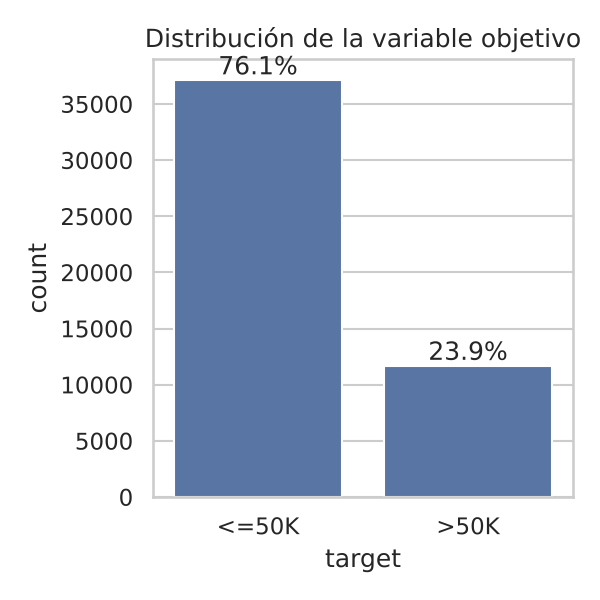
\includegraphics[width=\linewidth]{01_balance_clases.png}
        \caption{Distribución de la variable objetivo.}
    \end{minipage}\hfill
    \begin{minipage}[t]{0.54\textwidth}
        \centering
        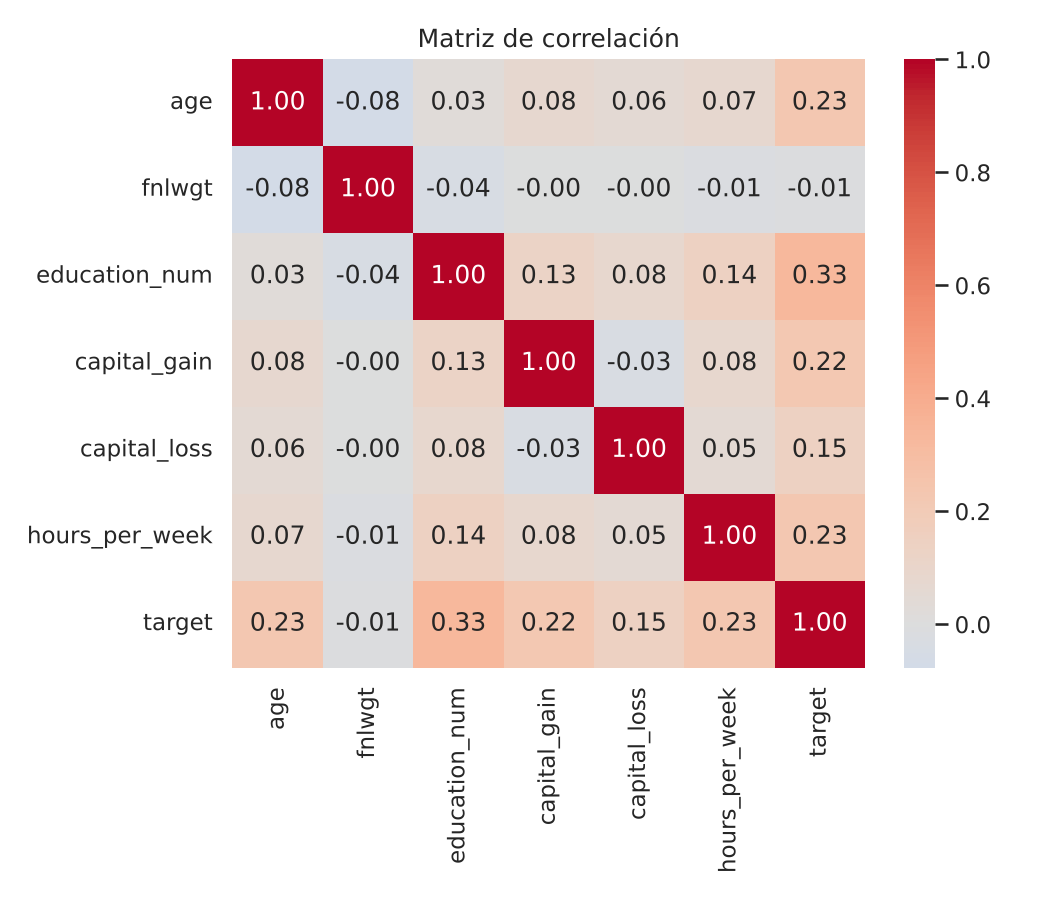
\includegraphics[width=\linewidth]{06_correlacion.png}
        \caption{Correlación entre variables numéricas.}
    \end{minipage}
    \fuente
\end{figure}

La distribución confirma el desbalance de clases. Frente al objetivo, las mayores correlaciones lineales son nivel educativo (0,33), edad (0,23), horas semanales (0,23) y ganancia de capital (0,22). Estas relaciones son moderadas; las variables categóricas también aportan información que la matriz de Pearson no representa.

\begin{figure}[H]
    \centering
    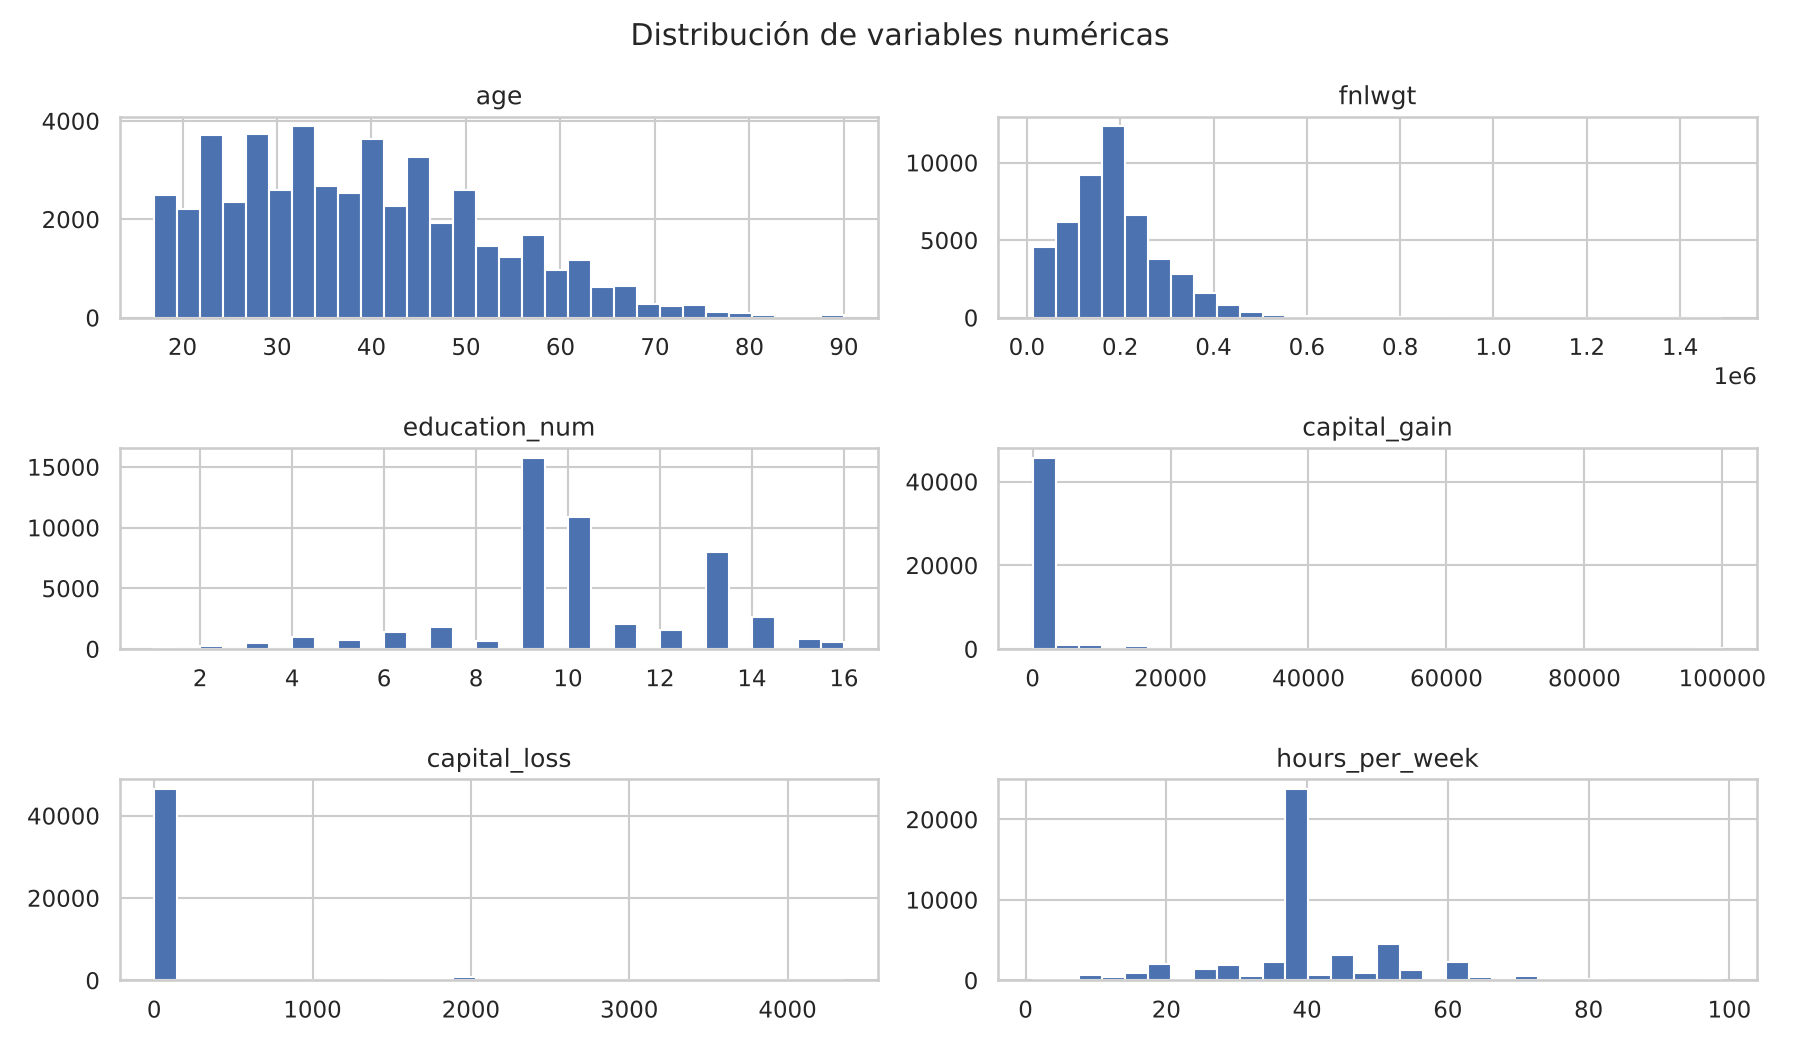
\includegraphics[width=0.83\textwidth]{02_hist_numericas.png}
    \caption{Distribución de las variables numéricas.}
    \fuente
\end{figure}

Los histogramas muestran asimetría fuerte en ganancias y pérdidas de capital, pues la mayoría de valores son cero, y dispersión en edad y horas trabajadas. Esto justifica transformar y escalar antes del entrenamiento.

\section{Preprocesamiento de la información}

Antes de transformar se divide el conjunto en entrenamiento y prueba de forma estratificada. Todas las estadísticas de preprocesamiento se calculan únicamente con entrenamiento para evitar fuga de información.

\begin{itemize}
    \item \textbf{Selección:} se elimina \texttt{education} porque duplica a \texttt{education\_num}. También se excluye \texttt{fnlwgt}, pues es un peso muestral y no una característica individual.
    \item \textbf{Variables categóricas:} las siete variables categóricas se convierten mediante codificación one-hot. Las columnas de prueba se alinean con las de entrenamiento. Así, la red recibe valores numéricos sin imponer un orden artificial entre categorías.
    \item \textbf{Valores nulos:} el símbolo ``?'' se interpreta como nulo. Aparece en \texttt{workclass} (5,73\,\%), \texttt{occupation} (5,75\,\%) y \texttt{native\_country} (1,75\,\%). Se imputa la moda calculada en entrenamiento, una decisión simple y adecuada por tratarse de variables nominales con pocos faltantes.
    \item \textbf{Normalización:} edad, nivel educativo, ganancias, pérdidas y horas semanales se estandarizan con z-score usando la media y desviación del conjunto de entrenamiento. Esto evita que las escalas mayores dominen el aprendizaje de la red.
    \item \textbf{Datos atípicos:} se detectan mediante boxplots y percentiles. Edad, horas, ganancias y pérdidas se limitan entre los percentiles 1 y 99 del entrenamiento, sin borrar personas válidas. Además, \texttt{capital\_gain} y \texttt{capital\_loss} reciben $\log(1+x)$ para reducir su asimetría.
\end{itemize}

\begin{figure}[H]
    \centering
    \begin{minipage}[t]{0.56\textwidth}
        \centering
        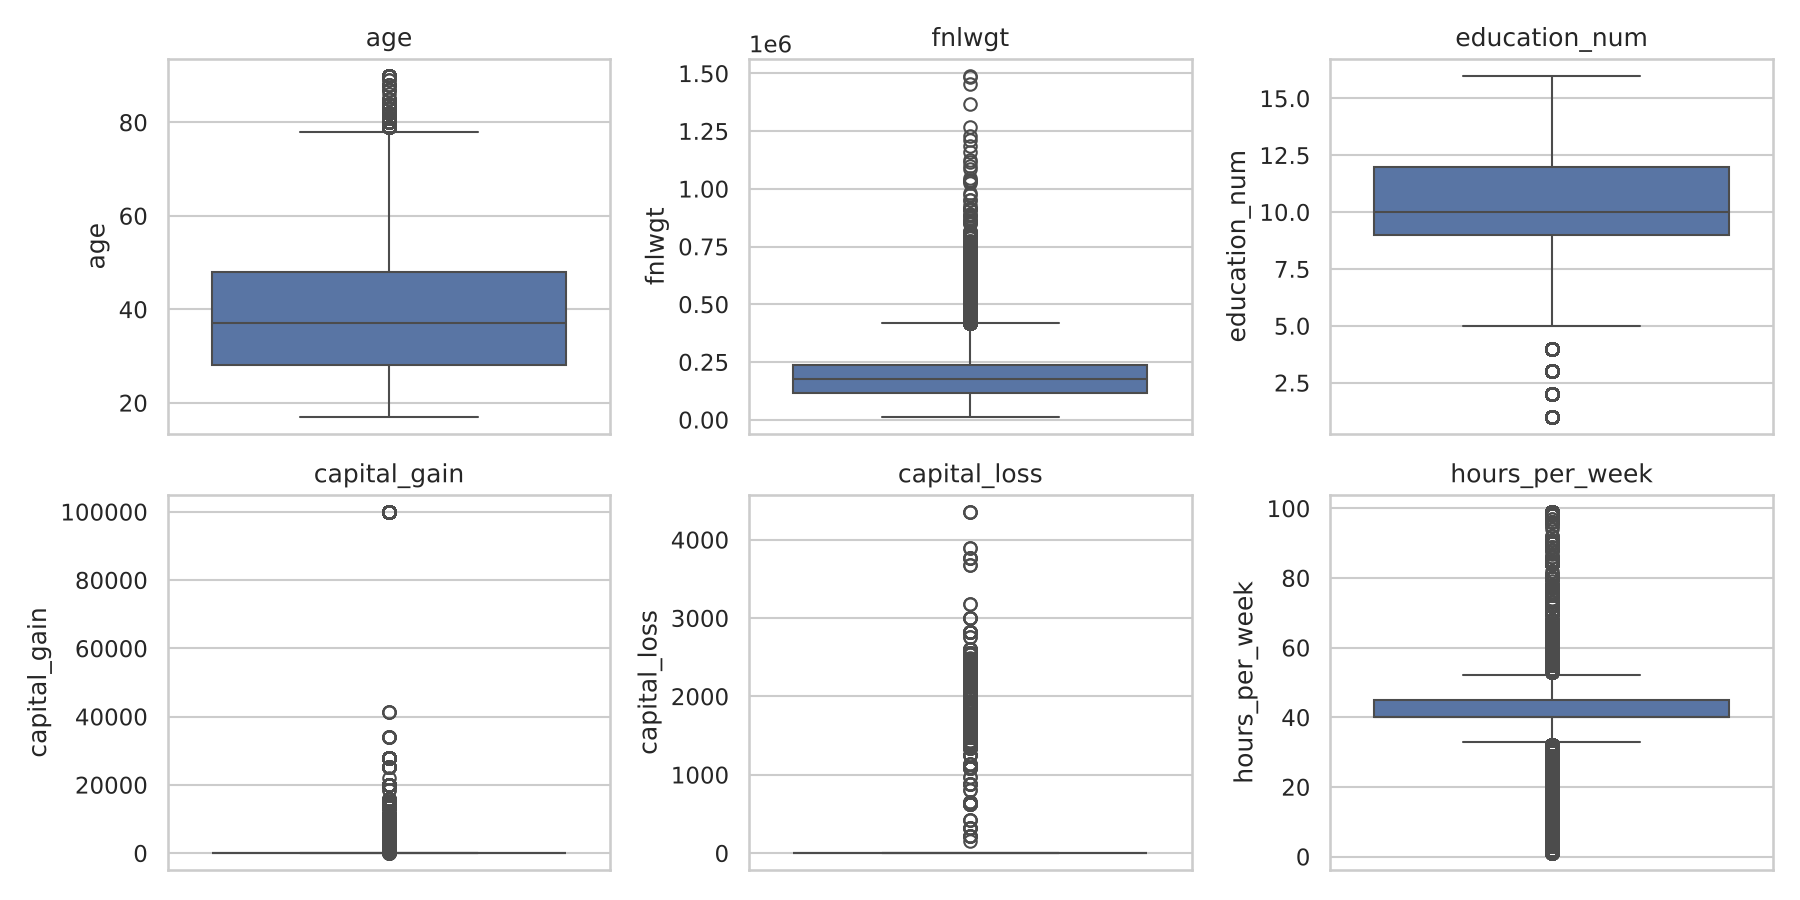
\includegraphics[width=\linewidth]{03_boxplots_outliers.png}
        \caption{Búsqueda de datos atípicos.}
    \end{minipage}\hfill
    \begin{minipage}[t]{0.40\textwidth}
        \centering
        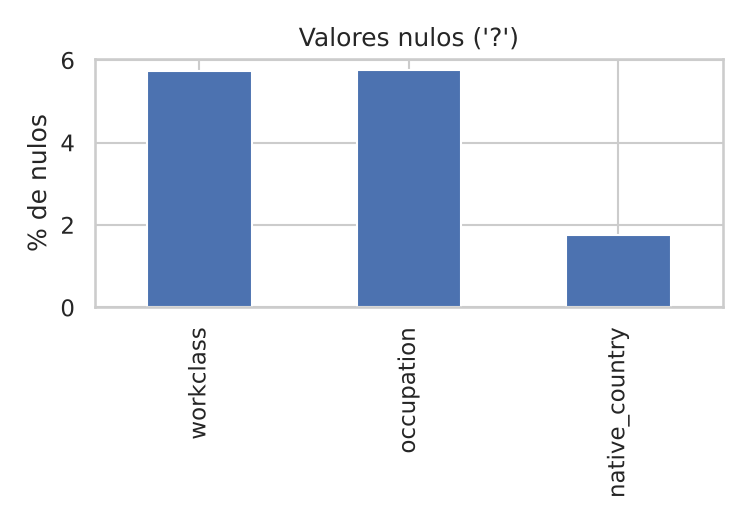
\includegraphics[width=\linewidth]{04_nulos.png}
        \caption{Porcentaje de valores nulos.}
    \end{minipage}
    \fuente
\end{figure}

El tratamiento conserva la mayor cantidad de observaciones, reduce el efecto de extremos y produce entradas numéricas comparables. La partición estratificada mantiene la proporción de clases; por el desbalance, la evaluación debe incluir precisión, exhaustividad y F1, además de exactitud.

\end{document}
